\chapter{Scepia}\thumbforchapter
\chapterauthor{Rebecca Snabel*, Maarten van der Sande*, Gert Jan Veenstra, Simon J. van Heeringen}
\newpage

\section{Introduction}

\begin{itemize}
    \item Enhancers important for cell type specification
    \item Transcriptomics vast growing field, many cell types sampled, chromatin accessibility assays remain behind (more costly, more sparse data): Difficulty in obtaining scChIP, scATAC still expensive for many labs
    \begin{itemize}
        \item  Many ChIP-seq experiments have been performed on tissues
    \end{itemize}
    \item SCEPIA only needs scRNA-seq input and uses available enhancer-ChIP data to infer cell type specific regulation
    \item HHCA provides a multiomic atlas of the heart
    \begin{itemize}
        \item Why is this atlas important?
    \end{itemize}
\end{itemize}

The state of a cell's gene activity is shaped by a complex network of genes and proteins, including transcription factors (TFs). TFs interact with each other and regulate the genes that they influence.

Transcriptomics has emerged as a rapidly expanding field, allowing researchers to explore the gene expression profiles of diverse cell types with increasing ease and affordability. However, when it comes to examining the accessibility or chemical modifications of chromatin, a crucial aspect of gene regulation, challenges persist. Single-cell ATAC-seq (scATAC), while immensely valuable, remains relatively costly and generates sparser data compared to transcriptomic methods. Single cell ChIP? Consequently, many laboratories encounter difficulties in adopting these techniques due to budget constraints and resource limitations. Bridging this gap in accessibility to chromatin-level data is vital for a more comprehensive understanding of gene regulation at the single-cell level and will likely be a focus of continued efforts in the field.

Recent advances in analyzing gene activity at the single-cell level offer exciting opportunities to understand how gene activity changes in detail. New statistical and computational methods tailored for single-cell gene analysis have led to valuable insights (XYZ). 

% However, it's still challenging to uncover the specific networks of genes and proteins that maintain stable cell states. This challenge arises because, at the single-cell level, gene activity can vary unpredictably due to factors like bursts of gene activity and other sources of randomness. While some methods can identify groups of genes that tend to be active together in single cells, they don't include an analysis of the regulatory signals that control how these genes are activated or suppressed by TFs.

\section{Methods}

\subsection{Data collection}

This is from ANANSE:
To generate a collection of putative enhancer regions, we collected all transcription factor ChIP-seq peaks from ReMap 2018 (\href{http://remap.univ-amu.fr/storage/remap2018/hg38/MACS/remap2018_all_macs2_hg38_v1_2.bed.gz}{http://remap.univ-amu.fr/storage/remap2018/hg38/MACS/remap2018\_all\_macs2\_hg38\_v1\_2.bed.gz}) (\href{javascript:;}{41}). We took the summit of all peaks and extended these 25 bp up- and downstream. Based on this file, we generated a coverage bedGraph using bedtools genomecov (\href{javascript:;}{78}). We performed peak calling on this bedGraph file using bdgpeakcall from MACS2 (version v2.7.1) (\href{javascript:;}{69}), with the following settings: \textit{l} = 50 and \textit{g} = 10. We performed the peak calling twice, setting \textit{c} to 4 and 30, respectively. All peaks from \textit{c} = 30 were combined with all peaks of \textit{c} = 4 that did not overlap with the peaks of \textit{c} = 30. We then removed all regions on chrM and extended the summit of the peaks 100 bp up- and downstream to generate a final collection of 1 268 775 putative enhancers of 200 bp. This collection of enhancers is available at Zenodo with doi 10.5281/zenodo.4066423.

Regulatory potential database was made by downloading all human bam files from ENCODE and mapping against REMAP.

Preprocessing of RNA-seq was done automatically by seq2science v1.0.3 \cite{seq2science} using the rna-seq workflow. Public samples were downloaded from the Sequence Read Archive \cite{Leinonen2010} with help of the ncbi e-utilities and pysradb\cite{Choudhary2019}. Genome assembly GRCh38.p13 was downloaded with genomepy 0.16.1 \cite{Frlich2023}. Paired-end reads were trimmed with fastp v0.23.2 \cite{Chen2018} with default options. Reads were aligned with STAR v2.7.10b \cite{Dobin2012} with default options. Afterwards, duplicate reads were marked with Picard MarkDuplicates v3.0.0 \cite{picard}. Bam files were converted to cram format with samtools samtools v1.16 \cite{Danecek2021}. Read counting and summarizing to gene-level was performed on filtered bam using HTSeq-count v2.0.2 \cite{Anders2014}. TPM normalized gene counts were generated using genomepy based on longest transcript lengths.

\subsection{Bulk regulatory potential comparison}

For the bulk 

\subsection{Single-cell comparison}


\subsection{Scepia}

\noindent
Input:

\begin{itemize}
	\item Reference database matrix of peak intensities (D) with dimensions (peaks x cell types). Scepia comes with multiple extensive reference databases, and user does not need to provide themselves.
    \begin{itemize}
    \item The peaks are REMAP
    \item The different cell types from ENCODE.
    \item The values are the quantile normalized log1p (IS THIS TRUE?) counts.
    \item H3K27ac, but can also be ATAC seq or ...
    \end{itemize}
	\item Single-cell RNA-seq dataset S with dimensions (cells x genes). 
    \begin{itemize}
        \item ...?
    \end{itemize}
\end{itemize}

% TODO TISSUE TYPES OR CELL TYPES? Or sth else?

\noindent
This is how scepia works:

\begin{enumerate}
    \item \textbf{Conversion of Reference Database Matrix}:
    
    Convert the reference database matrix of peak intensities $D$ into a database matrix of regulatory potential per gene $P$ with dimensions $(\text{genes} \times \text{cell types})$. The reference database includes all REMAP peaks, including promoters, and is prepared beforehand.
    
    \begin{itemize}
        \item The regulatory potential P of gene $g$ is calculated as:
        \begin{equation*}
            P_g = \sum_k w_{k}s_{k,g}
        \end{equation*}
        where $w_k$ is the weight at position $k$, and $s_{k,g}$ is the \textbf{log1p-transformed? TODO} h3k27ac signal at position $k$ for gene $g$.
        
        \item The weight function is calculated identically to ANANSE:
        \begin{equation*}
            w_k = \begin{cases}
                1, & \text{if } k \in (0\,\text{kb},\ 5\,\text{kb}] \\
                \frac{2e^{-\mu|k-t_g|}}{1+e^{-\mu|k-t_g|}}, & \text{if } k \in (5\,\text{kb},\ 100\,\text{kb}]
            \end{cases}
        \end{equation*}
        where parameter $t_g$ is the genomic position of the TSS of gene $g$, and $\mu$ determines the decay rate as a function of distance from the TSS, set such that an enhancer 10 kb from the TSS contributes one-half of an enhancer within 5 kb from TSS. $t_g$ is the distance from the TSS.
    \end{itemize}

    \item \textbf{Cell Annotation from Single-Cell Dataset}:
    
    Match cells in the single-cell dataset $S$ with regulatory potential $P$, resulting in an annotation matrix $A$ with dimensions $(\text{cells} \times \text{cell types})$. The transcript counts of each cell are regressed against the regulatory potential database (TODO, is x regressed against y, or vice versa?). The annotation matrix represents the regression coefficients, and cells receive a tissue/cell type annotation based on the highest regression coefficient.
    
    \begin{itemize}
        \item The first step involves selecting a subset of relevant cell types to speed up the cell annotation. It assumes that the user has already performed Louvain or Leiden clustering, and average counts are obtained per cluster. The top 2,000 most variable genes (dispersion normalized) are chosen. For each cluster $c$, the regression coefficients are calculated by lasso regression:
        \begin{equation*}
            S_c = P A_c + \lambda ||A_c|| + \epsilon
        \end{equation*}
        TODO I think this needs an $argmin(A_c)$.
        Absolute regression weights are summed per tissue/cell type, and only the (absolute) top 50 cell types/tissues are retained in the regulatory potential database.
        
        \item Mean center the single-cell counts and set each cell as the mean expression value of its neighbors. TODO, why no mean centering for regulatory potential? For each cell $i$, the regression coefficients are calculated using Bayesian ridge regression with the top 50 cluster weights:
        \begin{equation*}
            S_i = P A_i + \lambda ||A_i||^2 + \epsilon
        \end{equation*}
        Cells are initially assigned the cell type/tissue with the highest weight, and clusters are annotated based on the most common cell type in that cluster. Cell types are further refined by taking the dot product of cell type weights with neighborhood weights. Cell types require a minimum of 50 cells for assignment; otherwise, they are labeled as "other."
    \end{itemize}

    \item \textbf{Motif Scan over Differential Enhancers}:
    
    Look up the H3K27ac signal of the annotated cell types and retain the top 10,000 enhancers with the highest variance between them. The resulting matrix is denoted as $E$ and has dimensions $(\text{top X} \times \text{top Y})$. Conduct a (differential) motif scan over these enhancers. 
    
    \begin{itemize}
        \item Only known motifs are considered. 
        \item Motif scanning is done by Bayesian ridge regression
        \begin{equation*}
            \underset{\beta}{\operatorname{arg\,min}}\ \|y - X\beta\|^2 + \lambda \|\beta\|^2
        \end{equation*}
        TODO formula and TODO matrix names!
        TODO, the mean is subtracted here and I don't think it does anything meaningful...
    \end{itemize}
    

    \item \textbf{Calculation of Motif Scores}:
    
    Calculate the motif scores for the cells based on the motif scores of the reference top tissues. The motif scores per cell are calculated as a dot product of the cell type annotation weight and motif scores per reference tissue / cell type.
    \begin{equation*}
        F = S \cdot A
    \end{equation*}
    TODO check dimensions!

    \item \textbf{Correlation Analysis of Motif and Transcript Scores}:
    
    Determine significant combinations by correlating motif scores and transcript scores between cells:
    \begin{enumerate}
        \item Calculate the correlation coefficient between motif score and transcript counts.
        \item Randomly shuffle motif scores and calculate their correlation with transcript counts. Repeat this 100,000 times to obtain a distribution of correlation coefficients.
        \item Estimate two different p-values per TF-motif combination from this analysis: one based on the correlation coefficient relative to the total permuted set and another using only the permuted set of motif correlations. Combine these p-values using Fisher's method.
        \item Calculate motif activity by fitting a Gaussian mixture model with two components over the motif activity scores. These components represent "high" and "low" motif scores. Motif activity is computed as the probability that a motif score belongs to the "high" expressed group, and is thus constrained to the range of 0 to 1.
    \end{enumerate}
\end{enumerate}

% \begin{enumerate}
%     \item Convert the reference database matrix of peak intensities D into a database matrix of regulatory potential per gene (P) with dimensions (genes x cell types). The reference database includes all REMAP peaks, including promoters, and is made beforehand. 
%     \begin{itemize}
%         \item The regulatory potential of gene $g$ is calculated as: \begin{equation*}{P_{g}} = \sum\limits_k {{w_{k}}{s_{k,g}}\ } \end{equation*}
% where $w_k$ is the weight at position $k$ and $s_{k,g}$ the \textbf{log1p-transformed?} h3k27ac signal at position $k$ for gene $g$.
%         \item The weight function is calculated similar to ANANSE: \begin{equation*} w_k=\left\{\begin{matrix} 1, && k\epsilon (0\,{\rm kb},\ 5\,{\rm kb}]\\ \frac{2{\rm e}^{-\mu|k-t_g|} }{1+{\rm e}^{-\mu|k-t_g|}}, && k\epsilon (5\,{\rm kb},\ 100\,{\rm kb}] \end{matrix}\right. \end{equation*}
% where parameter $t_g$ is the genomic position of the TSS of gene $g$, and $\mu$ determines the decay rate as a function of distance from the TSS, is set such that an enhancer 10 kb from the TSS contributes one-half of an enhancer within 5 kb from TSS. $t_g$ is the distance
%     \end{itemize}

%     \item Match cells in the single-cell dataset (S) with regulatory potential (P) resulting in annotation matrix A with dimensions (cells x cell types). The transcript counts of each cell are regressed against the regulatory potential database. The annotation matrix is thus the regression coefficients. Cells get a tissue/celltype annotation based on the highest regression coefficient.
%     \begin{itemize}
%         \item The first step is to take a subset of the relevant cell types as regression on the whole dataset is slow. It expects that the user already did Louvain or Leiden clustering, and the average counts are taken per cluster. The top 2,000 most variable genes (dispersion normalized) are taken. For each cluster $c$, the regression coefficients are then calculated to  $S_c = P A_c + \lambda ||A_c|| +\epsilon$. Absolute regression weights are taken, summed per tissue/cell type. Only the top 50 cell types/tissues are kept in the regulatory potential database.
%         \item Mean center the single cell counts, and set each cell as the mean expression value of its neighbours. For each cell $i$, the regression coefficients are calculated as bayesian ridge regression, with the top 50 cluster weights: $S_i = P A_i + \lambda ||A_i||^2 +\epsilon$. Cells are initially assigned the cell type / tissue with the highest weight. Clusters are then annotated by the most occurring cell type. Cell types are then re-estimated by taking the dot product of the cell type weights by the neighbourhood weights. Cell types need a minimum of 50 cells to be assigned to otherwise assigned "other". 
%         \item \textbf{TODO why lasso and then ridge?!}
%     \end{itemize}

%     \item Look up the H3K27ac signal of the annotated cell types, and keep the top 10,000 enhancers with the highest variance between them. E with dimensions (top X x top Y).

%     \item Do a (differential) motif scan over the differential enhancers. Only known motifs 
%     \begin{itemize}
%         \item We do a Bayesian ridge regression to infer the motif weights TODO formula: $S_i = P_i A_i + \lambda ||A_i||^2 +\epsilon$
%         \item TODO ridge is $ \underset{\beta}{\operatorname{arg\,min}}\; \|y - X\beta\|^2_2 + \lambda \|\beta\|^2_2 $
%     \end{itemize}
    
%     \item dot product of annotation weights and motif scores F
%     \begin{itemize}
%         \item $F = S \cdot A$ needs to be checked for dimensions!
%     \end{itemize}

%     \item Correlate motif scores and transcript scores between cells. This is used to determine significant combinations.
%     \begin{enumerate}
%         \item Calculate the correlation coefficient between motif score and transcript counts. 
%         \item Then randomly shuffle motif scores, and calculate their correlation with the transcript counts. Repeat this 100,000 times to get a distribution of correlation coefficients.
%         \item Now we estimate two different p-values from this, by taking the correlation coefficient relative to two distributions of correlation coefficients. The first correlation coefficient distribution is the total permutated set, and the second distribution is only the permutated set of the motif. The p-values are then combined by fisher's method.
%         \item \textbf{WHY?}
%         \item Motif activity is calculated by fitting a gaussian mixture model with two components over the motif activity scores. These components than represent the "high" and "low" motif scores. The motif activity is calculated as the probability that a motif score belongs to the "high" expressed group. This makes it so that the motif activity score is limited between 0 and 1.
%     \end{enumerate}
% \end{enumerate}

\section{Results}

\subsection{Matching regulatory potential and RNA}

To examine the relationship between regulatory potential and RNA-seq, we downloaded X human RNA-seq cell types and Y human H3K27ac cell types from ENCODE. We then calculated the correlation coefficient between all combinations of regulatory potential and RNA-seq TPM (Fig. \ref{fig:celltypes}). The average correlation coefficient between the same cell types is $0.53 \pm 0.14$, and in $64\%$ of the cases, the regulatory potential of a tissue had the highest correlation coefficient with the TPM of the same tissue type. Broadening XXX resulted in a $77\%$ correct annotation. The exact parameters for the calculation of the regulatory potential do not particularly matter, as the signal in the promoter is enough to predict TPM. As such we think that the H3K27ac regulatory potential signal is an acceptable classifier for cell state.
\begin{figure}
    \centering
    \includegraphics[width=0.75\linewidth]{ch.scepia/imgs/celltypes.png}
    \caption{Ill encircle some stuff for convincing. Not sure which cmap, all are ugly.. or not colorblind, or red green and thats confusing microarray. Also Ill remove labels in the end?}
    \label{fig:celltypes}
\end{figure}
The relationship between RNA-seq and regulatory potential led us to the question of whether transcriptomic data is capable of predicting transcription factor motif activity / scores, and whether a reference database of H3K27ac would improve this. To estimate this we took subsets of five tissues/cellt types present in both our H3K27ac reference database and transcriptomic dataset. We established a ground truth by doing a motif scan on the top 25,000 most differential enhancers. A naive approach would assume that the TPM of a transcription factor one-to-one translates to its motif score. As shown in figure \ref{fig:bulk_benchmark} the naive approach correlates extremely poorly with our ground truth. A regulatory potential based approach would first translate the TPMs into RP. We then regress the most important cell types, take their top 10,000 most differential enhancers, and do a motif scan on those. We then multiply the motif scores with the cell type / tissue weights to get a motif score for original. This is a major improvement over the naive approach (Fig. \ref{fig:bulk_benchmark}). 


To establish the sensitivity to the peaks chosen we compared that to the top 10,000 most differential enhancers.  

\begin{figure}
    \centering
    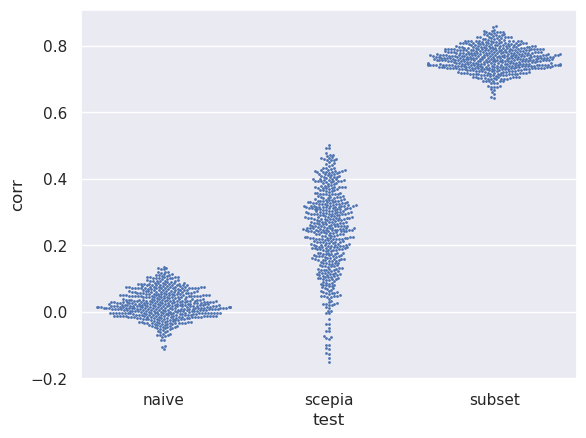
\includegraphics[width=0.75\linewidth]{ch.scepia/imgs/scepia_bulk_benchmark.png}
    \caption{scepa -> regulatory potential based inference}
    \label{fig:bulk_benchmark}
\end{figure}
See supplemental figure XXX for parameter sweep. This is nice because test/validate separate

\subsection{Single-Cell Epigenome-based Inference of Activity}

\begin{figure}
    \centering
    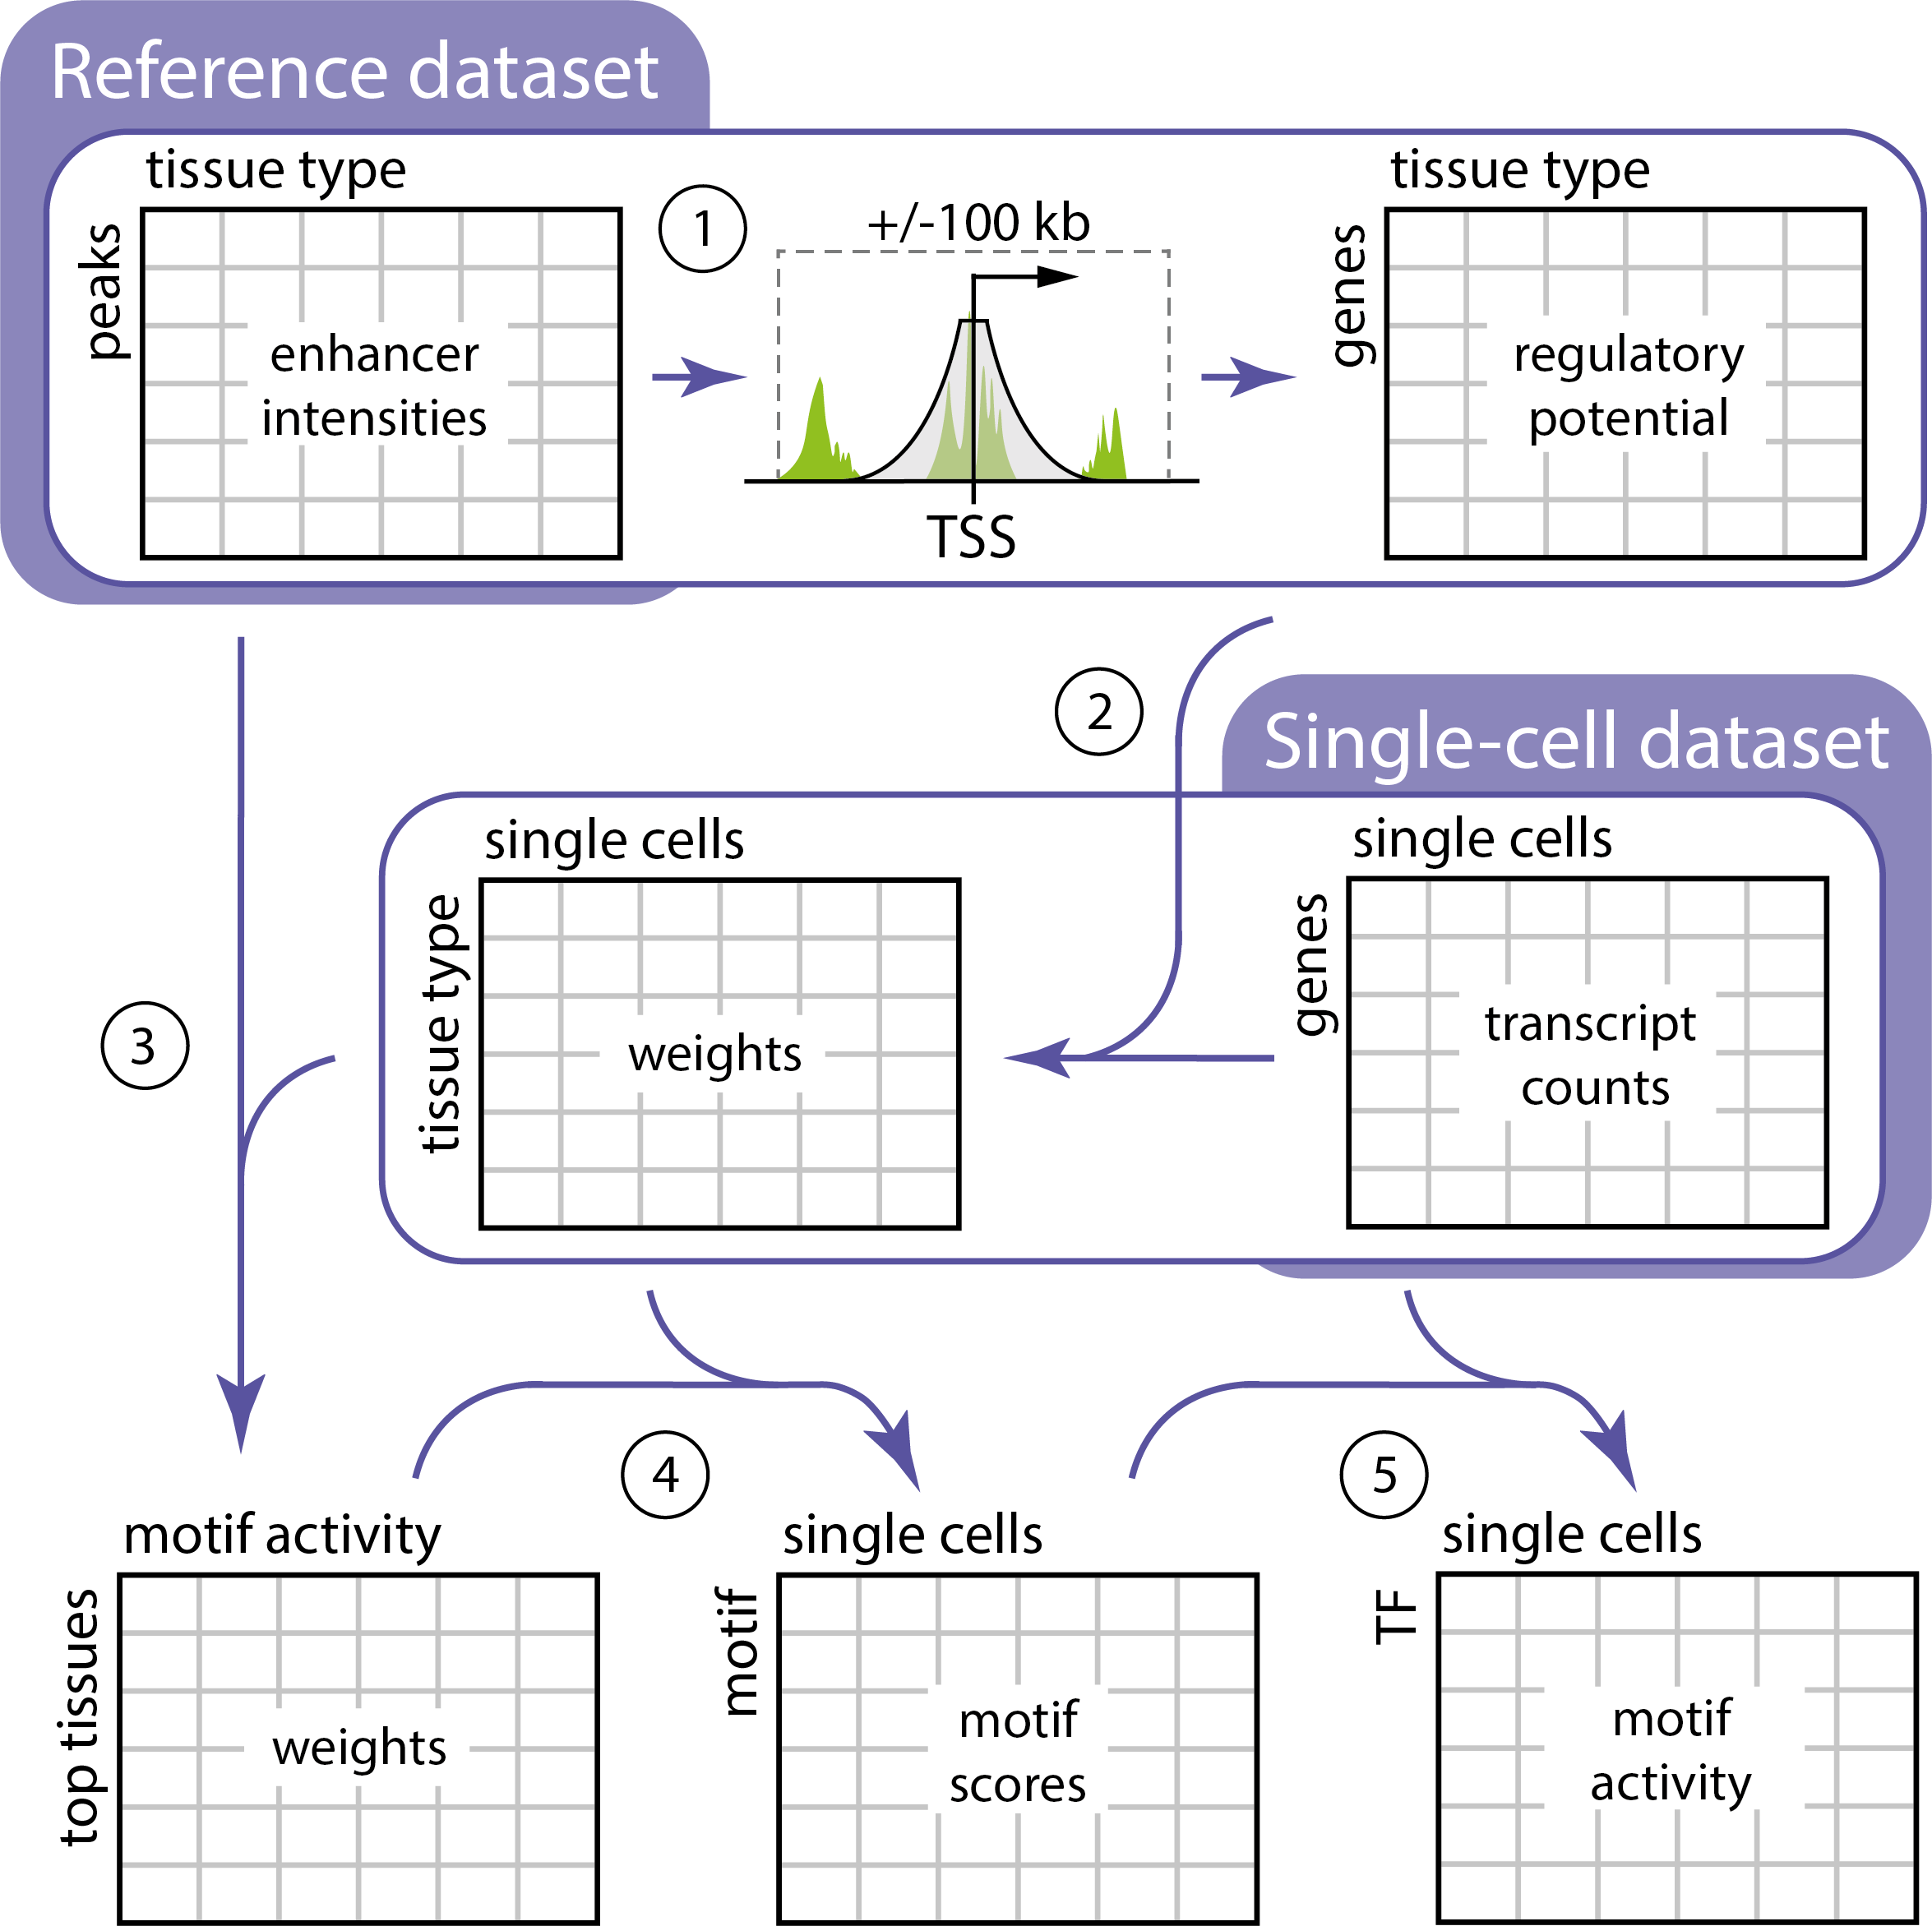
\includegraphics[width=1\linewidth]{ch.scepia/imgs/Middel 6OverviewFigureNumbers.png}
    \caption{\textbf{Scepia matches X Y Z}, TODO}
    \label{fig:enter-label}
\end{figure}


\textbf{SCEPIA on HHCA scRNA-seq data: }
How did the annotation work, overal hits with motifs???, some examples of single-cell motif activity plotted onto UMAP
\begin{figure}
    \centering
    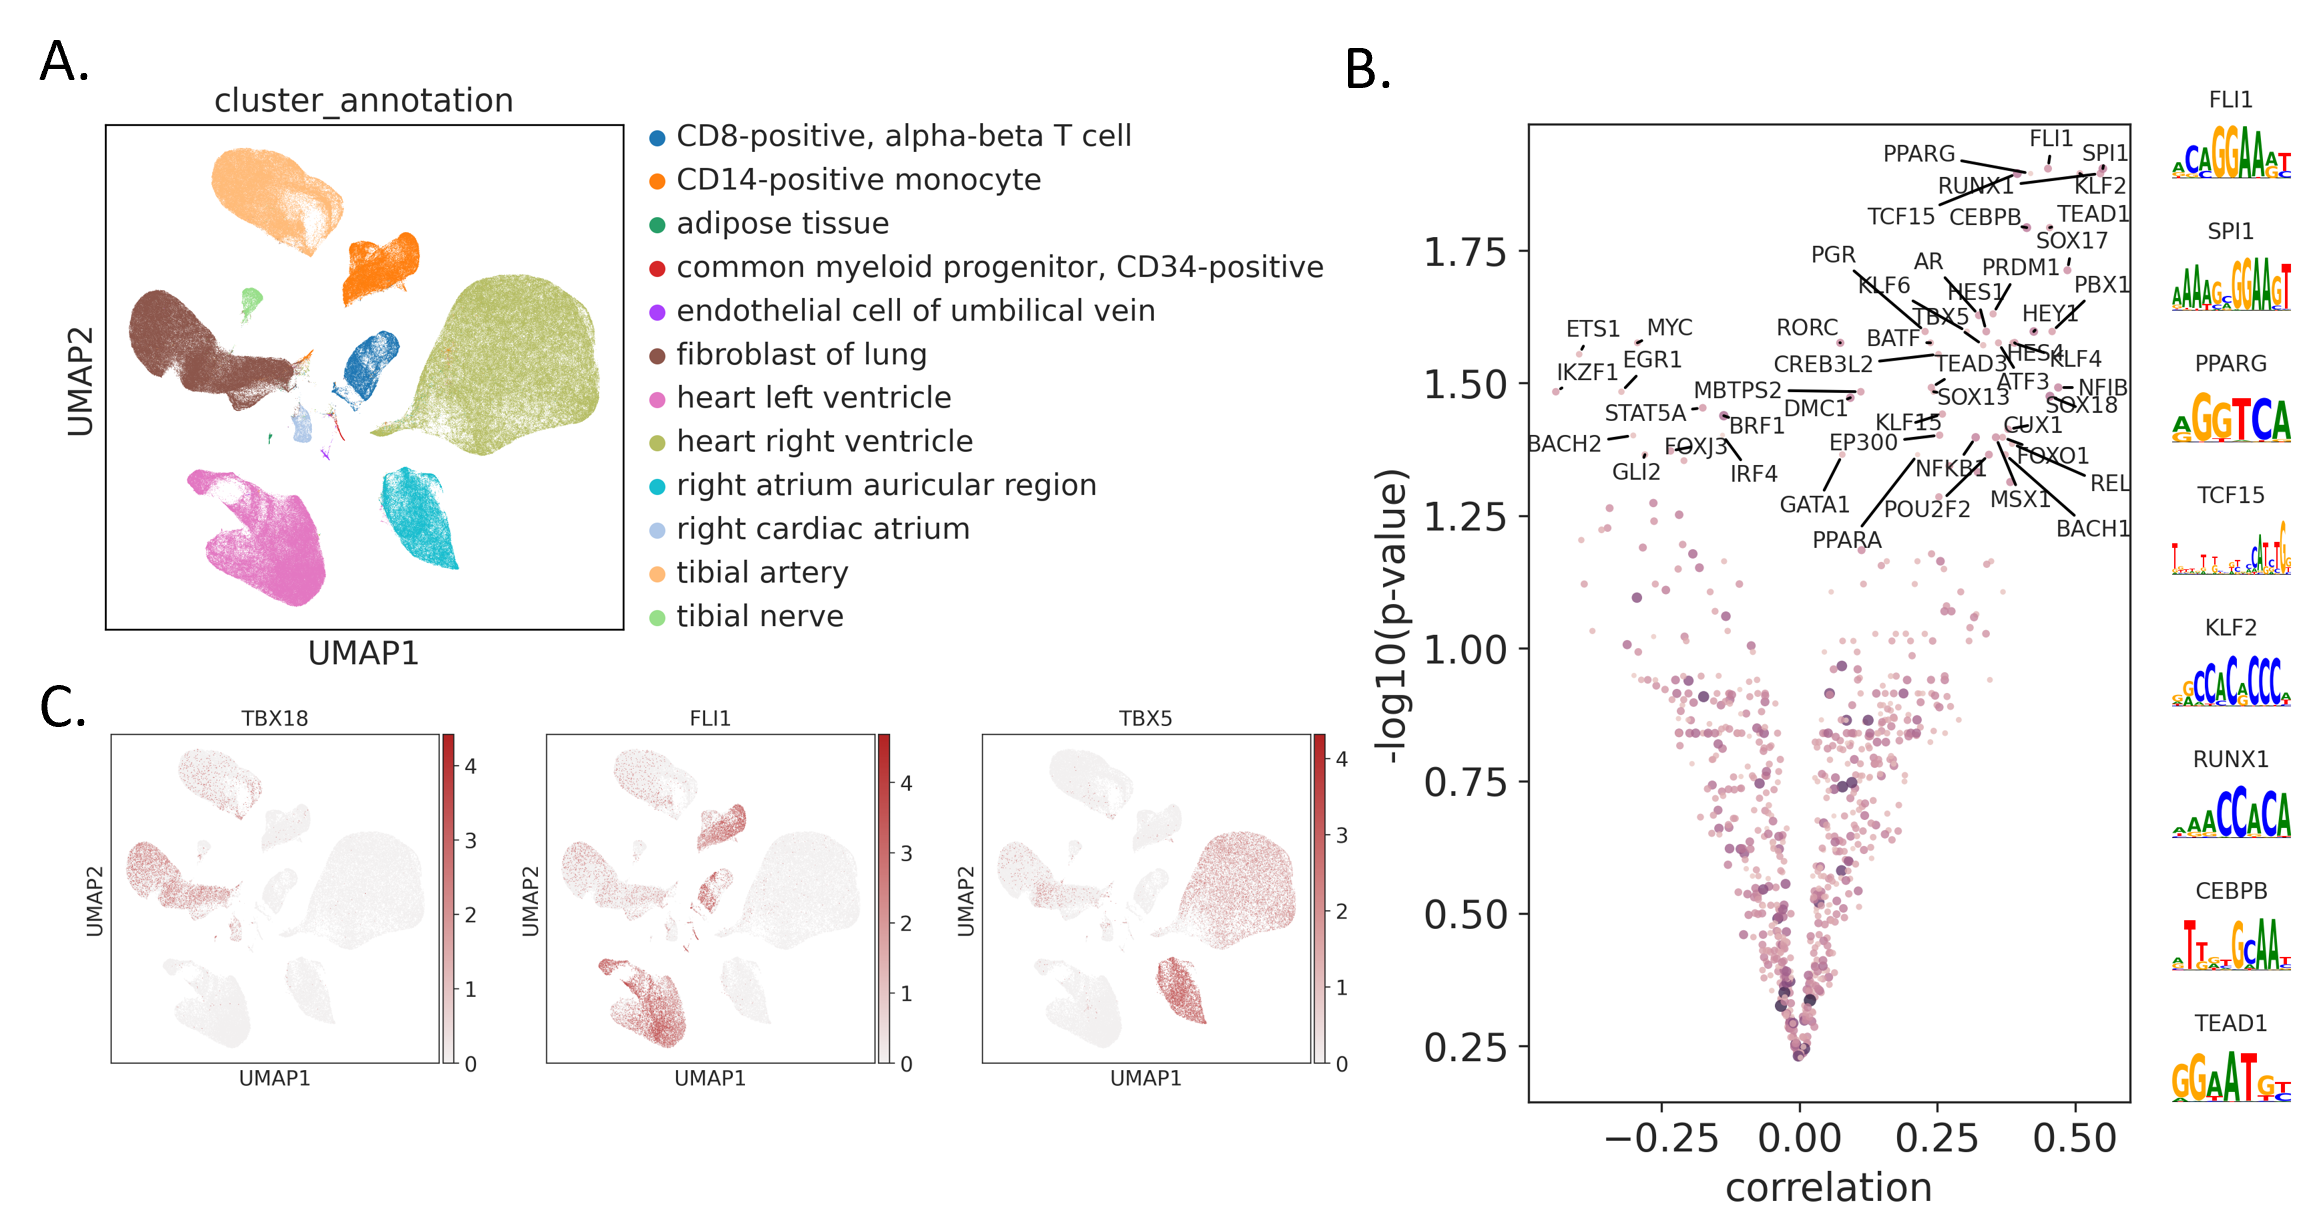
\includegraphics[width=0.75\linewidth]{ch.scepia/imgs/SCEPIAonHHCA.png}
    \caption{SCEPIA run on the Human Heart Cell Atlas}
    \label{fig:scepia_hhca1}
\end{figure}

% \hvFloat[doublePage,capWidth=n,
% capPos=bottom,bindCorr=0.0cm]{figure}
% {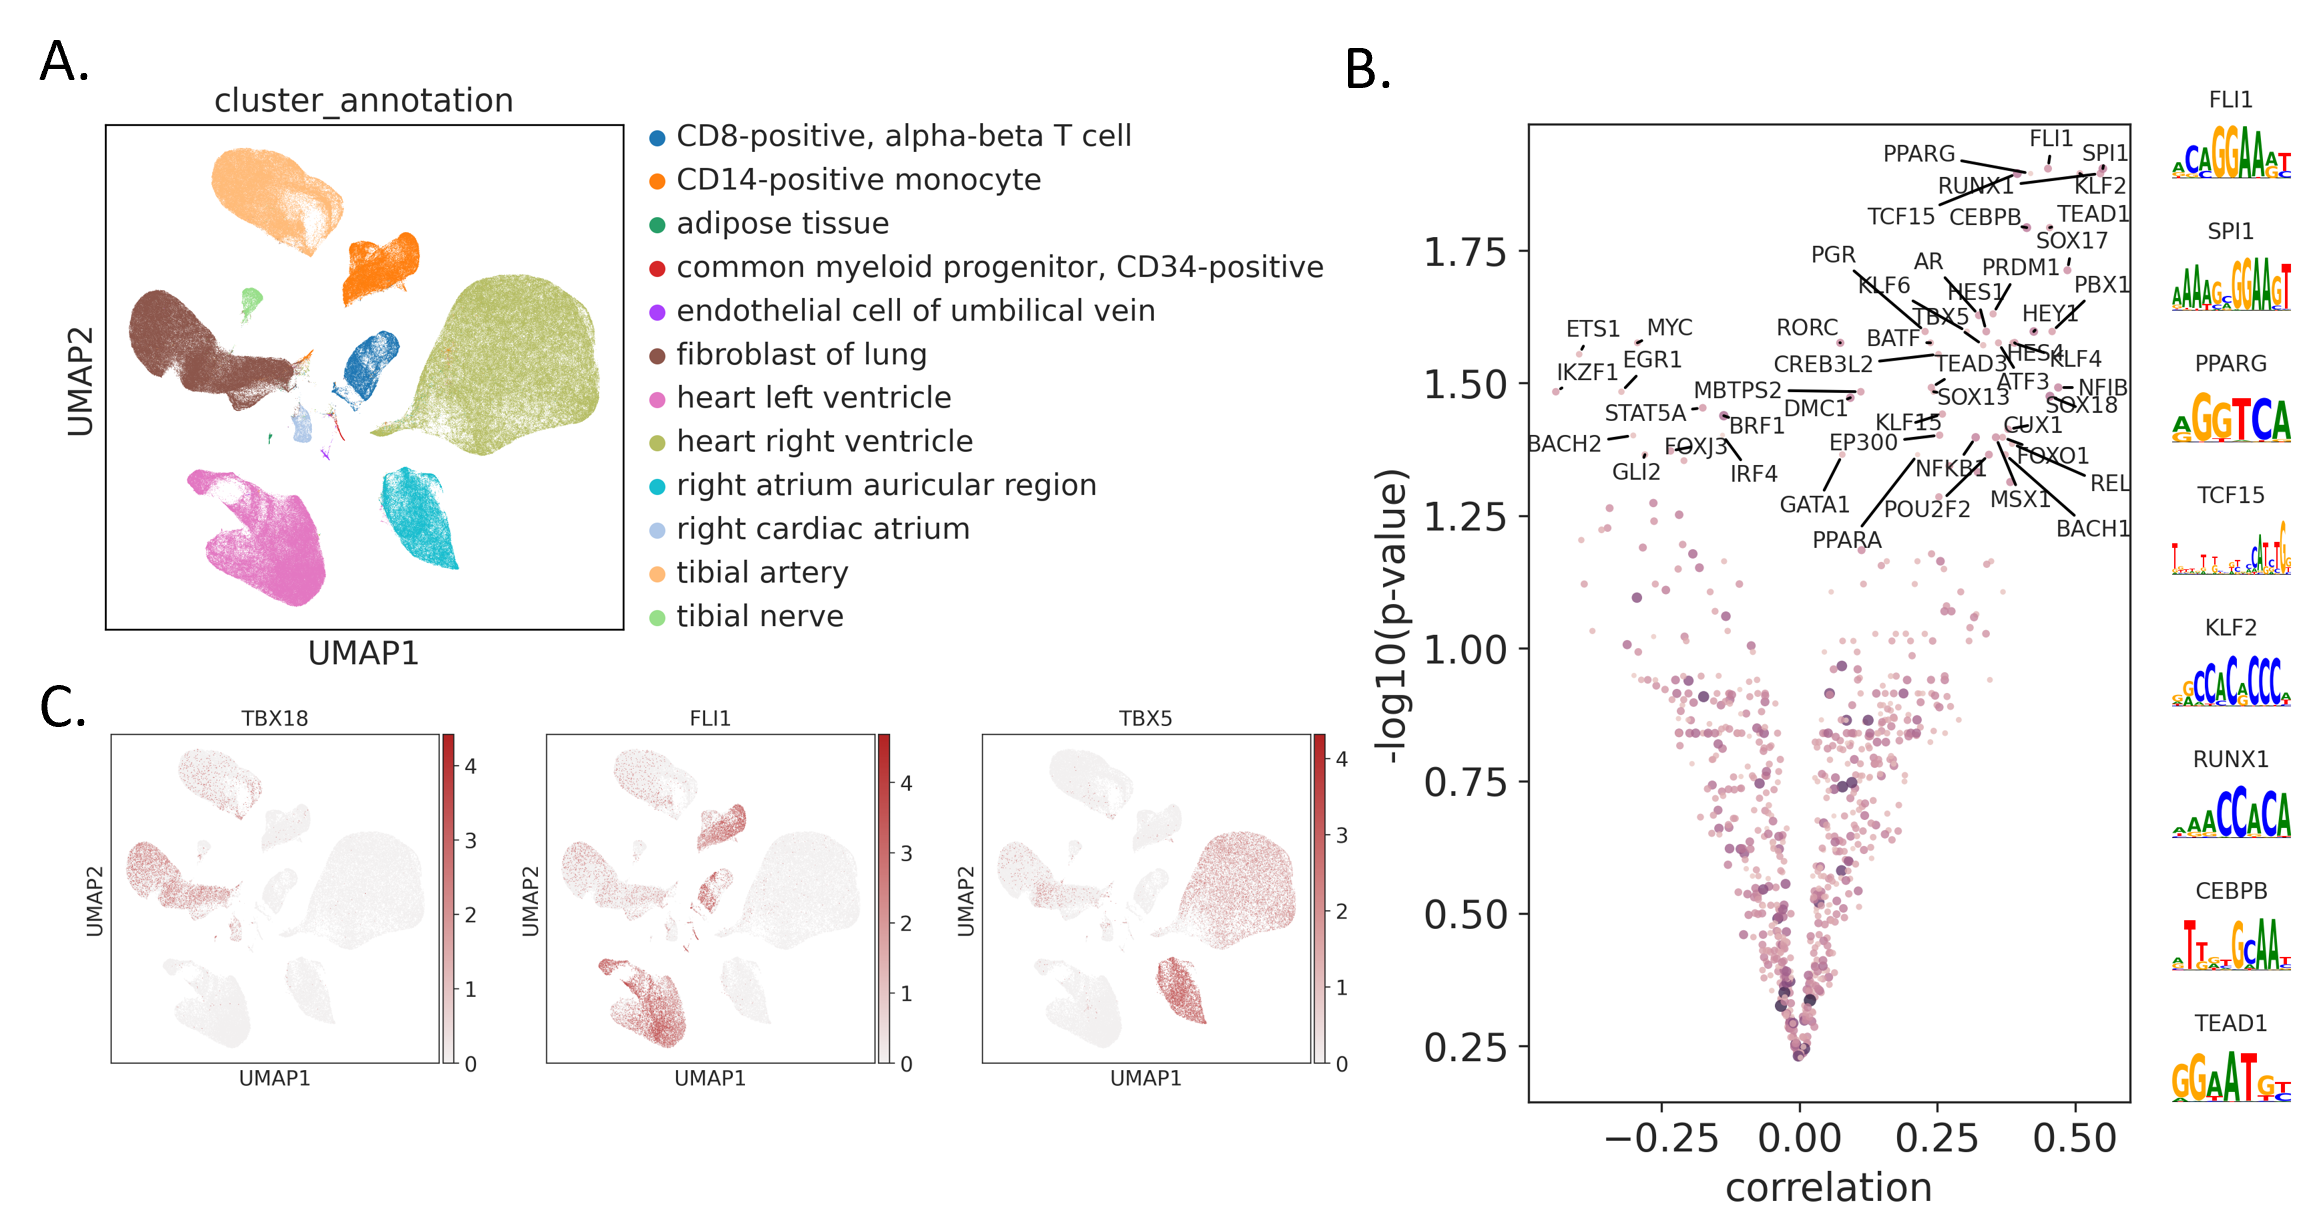
\includegraphics[width=1.6\textwidth]{ch.scepia/imgs/SCEPIAonHHCA.png}}
% [blabla]
% {SCEPIA run on the human heart cell atlast}{fig:scepia_hhca}


Probably merged with figure below: Cluster averaged motif activities for SCEPIA top hits; compared to motif activity per cluster as called on the ATAC-profiles.

\begin{figure}
    \centering
    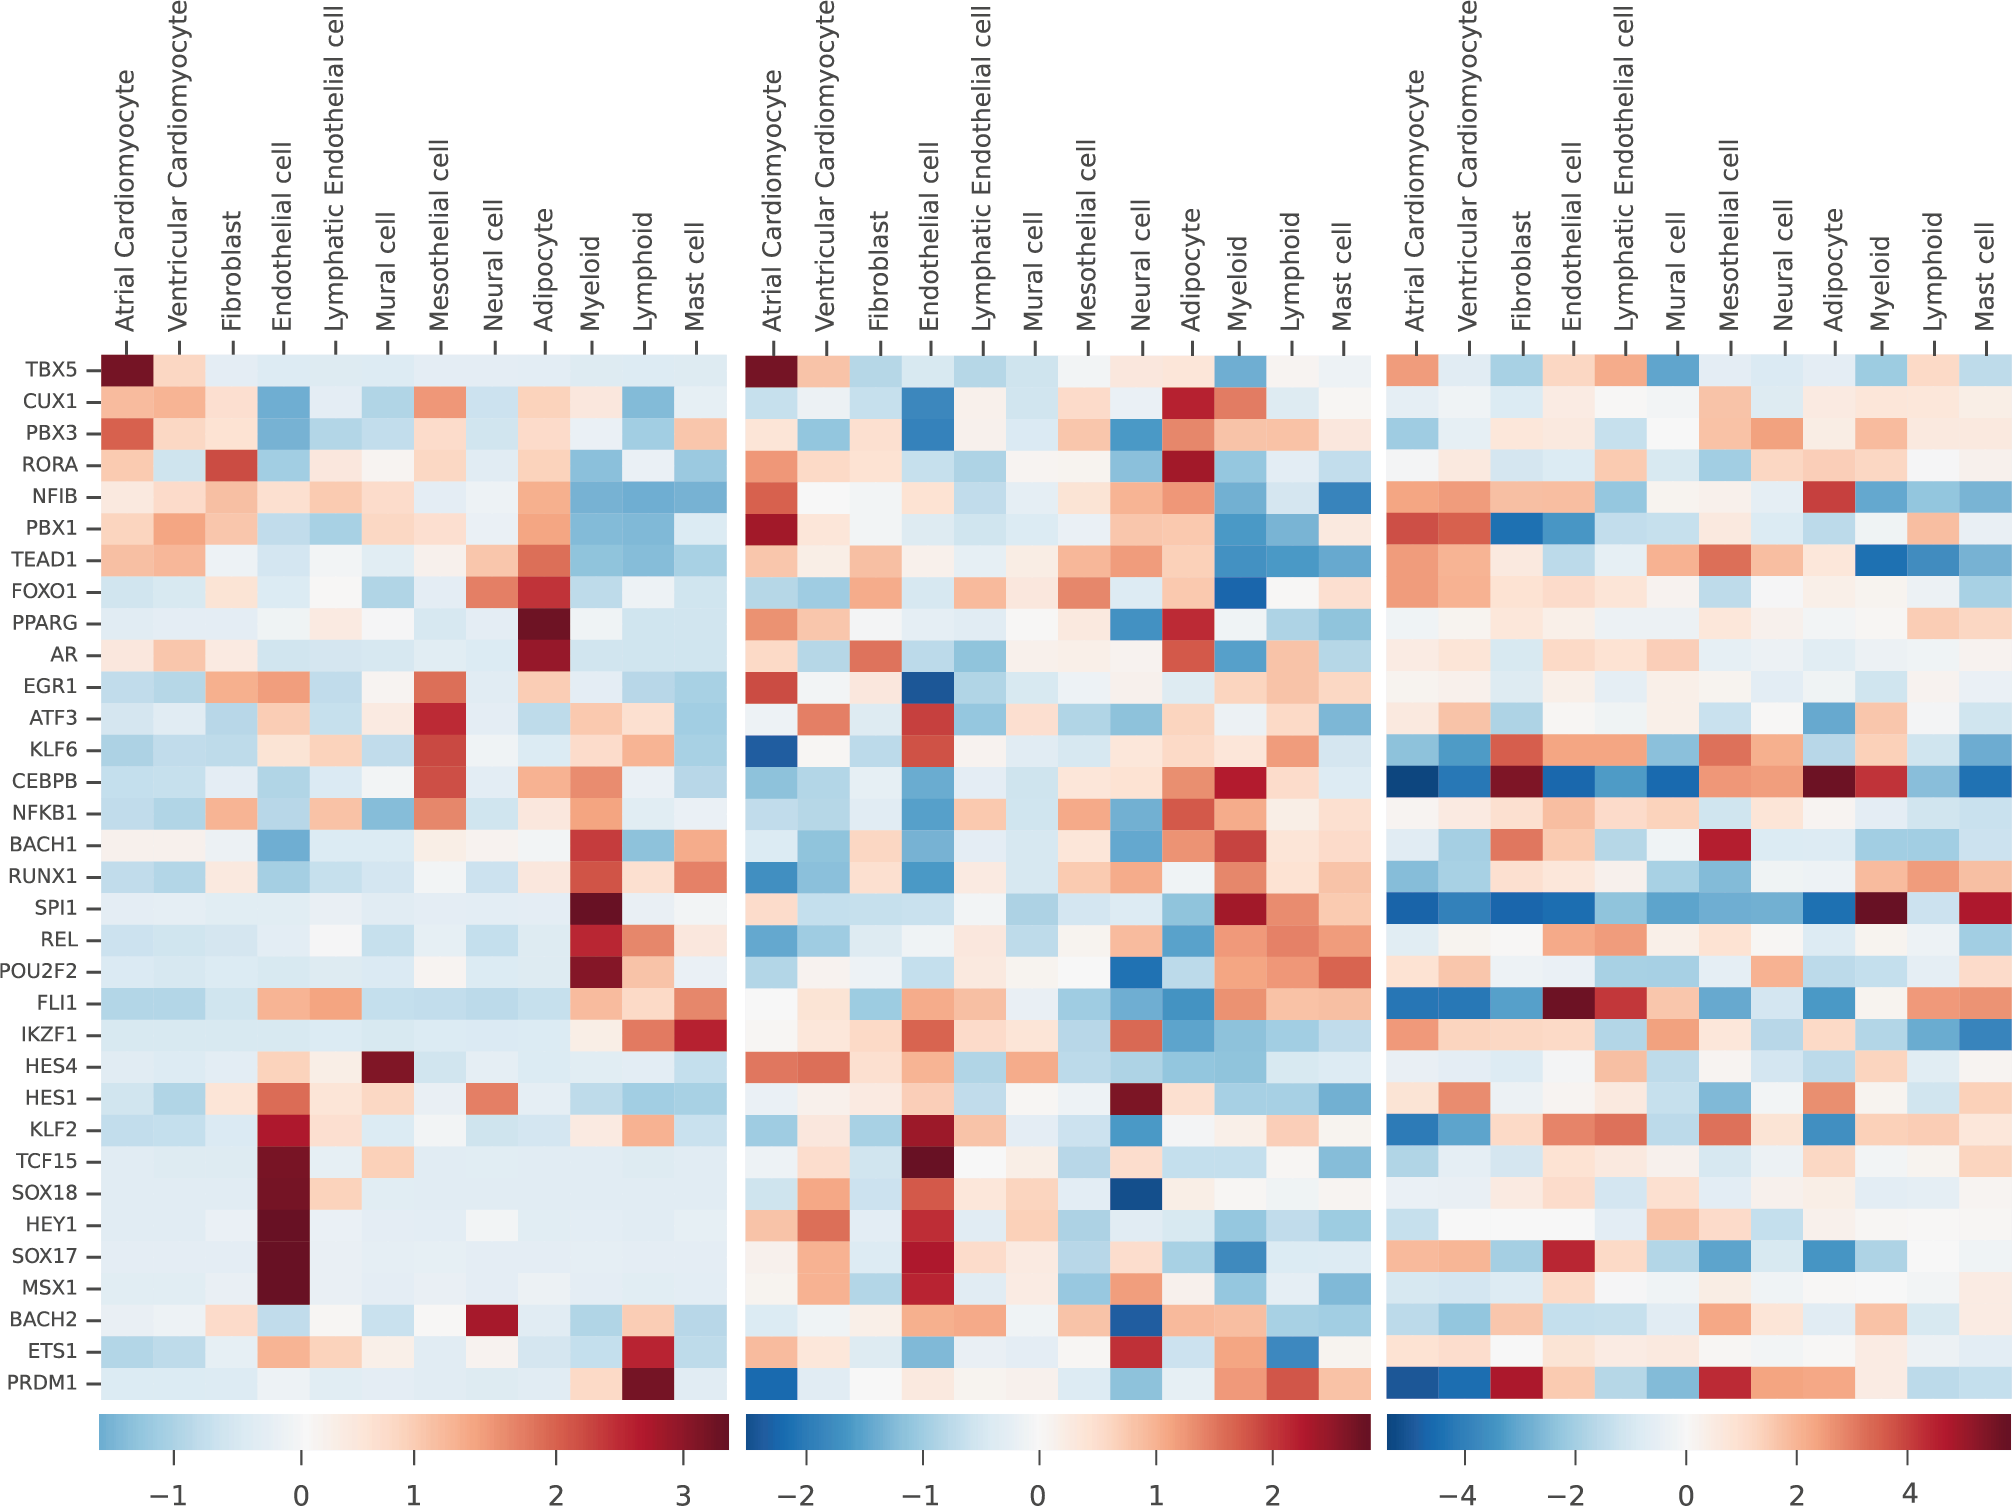
\includegraphics[width=0.75\linewidth]{ch.scepia/imgs/Middel 1SCEPIAhitsHHCA.png}
    \caption{SCEPIA hits, left: Expression levels TFs, middle: Motif activity per TF predicted by SCEPIA, right: Maelstrom motif activity for these same motifs, ran on scATAC peak intensities per cell type
    }
    \label{fig:scepia_hhca2}
\end{figure}

Comparing SCEPIA with Maelstrom motif activities
\textit{-> 1 large cluster of adipocyte expressed factors (RORA-[...]-AR) that have no expression in the immune cell types (Myeloid, Lymphoid, Mast cell), show an irregular pattern of accessibility in the ATAC data for the immune cells. (OR the protein is still there and its not measured in the RNA levels) Combining the motif accessibility with the expression levels of their binding targets, shows a specificity of these factors for the adipocytes (and some in CM) which was not picked up in the maelstrom analysis.\href{https://www.cell.com/molecular-cell/fulltext/S1097-2765(00)80209-9?_returnURL=https\%3A\%2F\%2Flinkinghub.elsevier.com\%2Fretrieve\%2Fpii\%2FS1097276500802099\%3Fshowall\%3Dtrue}{PPAR gamma is required for placental, cardiac, and adipose tissue development }}

\textbf{NEEDED FIGURE???}
SCEPIA on 100K subsets of HHCA scRNA-seq versus naive correlations between Maelstrom motif activity and binding gene expression levels
SCEPIA with and without geosketch filtering: \textbf{check for interesting biology} -> Otherwise \textit{maybe} supplemental.
\begin{figure}
    \centering
    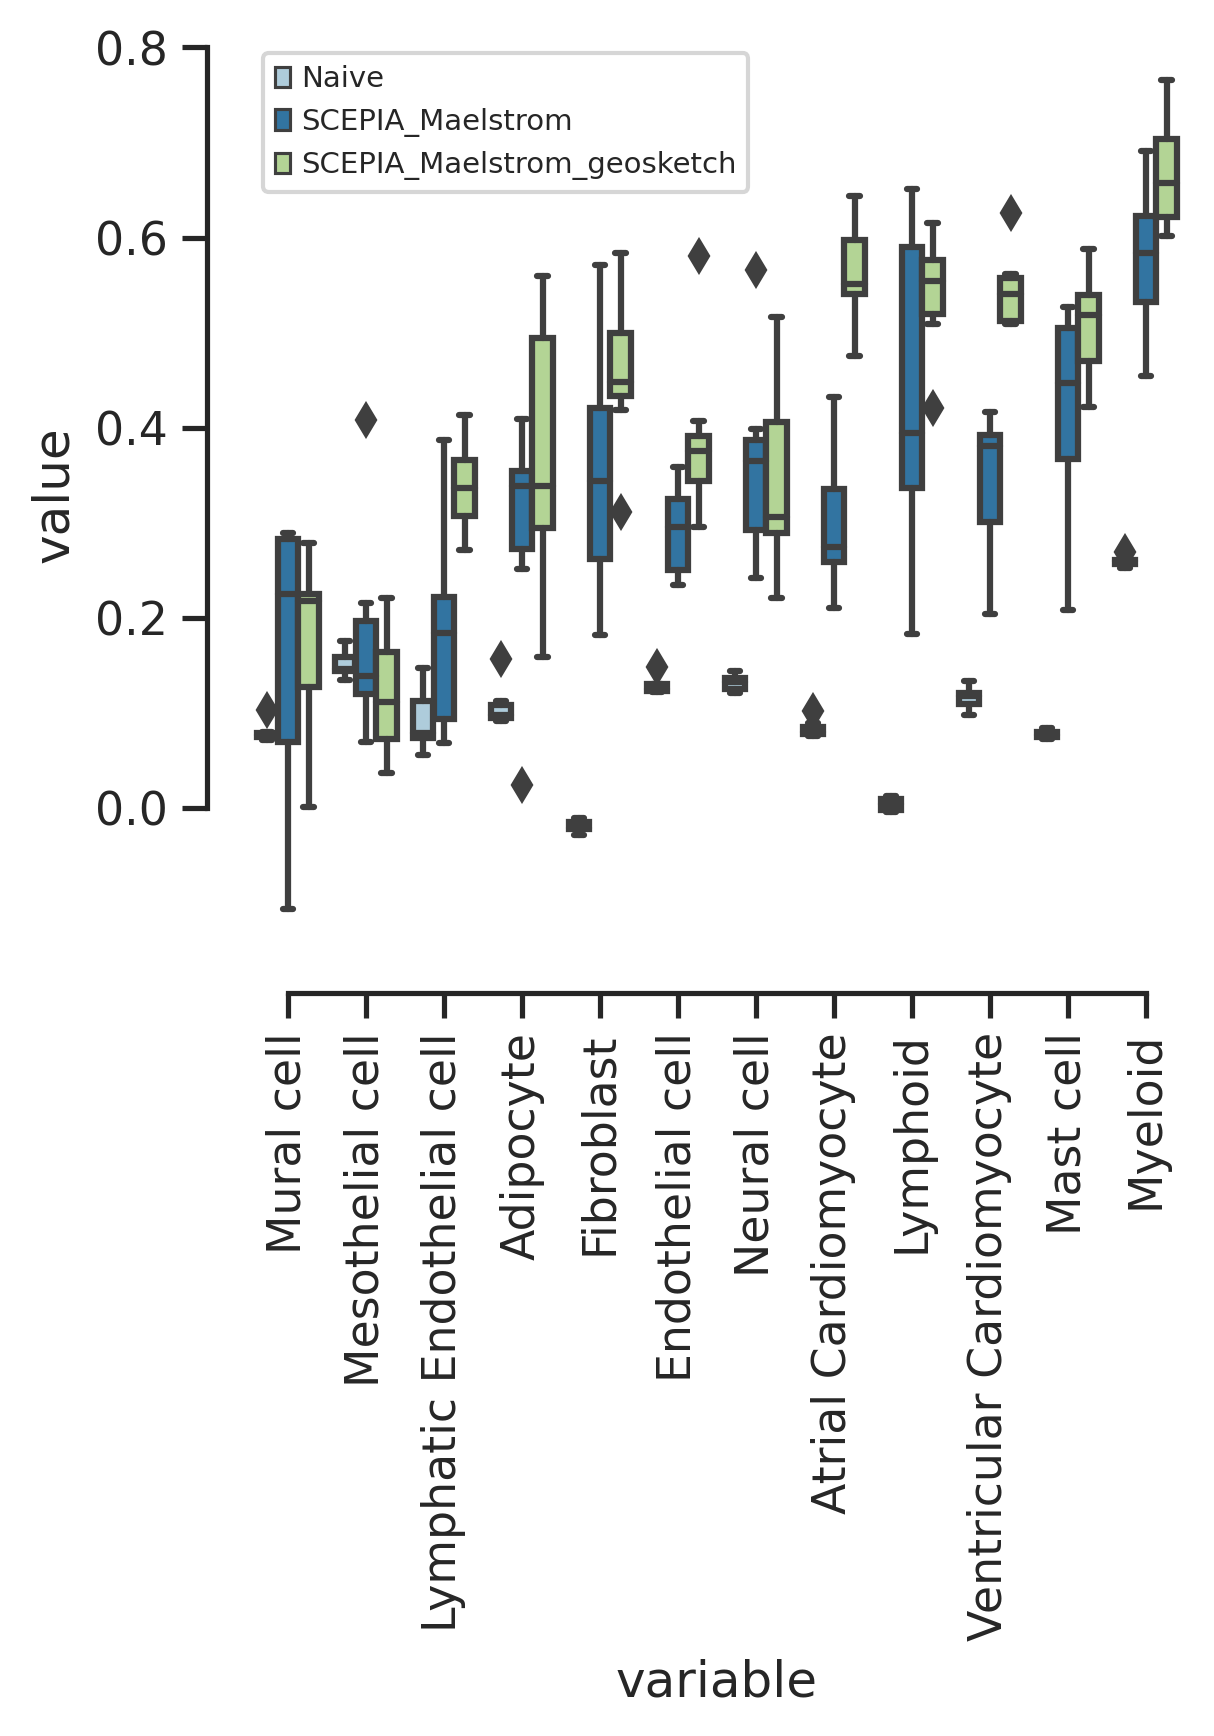
\includegraphics[width=0.75\linewidth]{ch.scepia/imgs/CorrelationsGeosketch_perCT.png}
    \caption{SCEPIA sc benchmark - Geosketch}
    \label{fig:sc_benchmark}
\end{figure}

\section{Discussion}

\subsection{Limitations}
\begin{itemize}
    \item Benchmark is bad. Benchmarking against a bad ground truth is stupid.
    \item Can not detect alternative splcing / rna degradation / post translational modificaitons etc.
    \item Why do we use ridge / lasso? Why not elasticnet?
\end{itemize}

\section{Supplementals}
\beginsupplement
\begin{table}
\begin{center}
\begin{tabular}{||c c c c||} 
\hline
Weight curve & Correlation between & Correct specific & Correct broad \\[0.5ex] 
\hline
Ananse & $0.53 \pm 0.14$ & $64\%$ & $77\%$ \\ 
\hline
Wang & $0.54 \pm 0.15 $ & $64\%$ & $75\%$ \\
\hline
Promoter (5kb) & $0.54 \pm 0.14$ & $66\%$ & $77\%$ \\
\hline
Enhancer & $0.43 \pm 0.14$ & $60\%$ & $72\%$ \\
\hline
\end{tabular}
\caption{Caption of my table.}
\label{table:1}
\end{center}
\end{table}
